\subsection{Initial implementation}

The initial implementation of a Great Lakes model based on NOAA/NCEP's WAVEWATCH
III code (henceforth the GLW model), begun in late 2004. During the first three
quarters of 2005, a wave forecasting system
using WAVEWATCH III was developed and tested, and by late 2005, a
pre-operational version of the GLW model was deployed. In June 2006, an
experimental web site made available
the four-times daily GLW forecasts for public access. In August 2006,
the experimental GLW system was made operational within the US National
Weather Service suite of numerical weather prediction models. 

In this section, a brief overview of the work undertaken in this first, initial
implementation period is provided.

\subsubsection{Spectral resolution}

In the major oceanic basins, waves can develop over long fetches and propagate
long distances, originating wave-energy spectra that may contain significant
amounts of energy in very low frequencies (eg, of the order of 0.04Hz).
Therefore, typical wind-wavel models use discrete energy spectra with
frequencies ranging from 0.04Hz up to 0.5Hz. The confined nature of the lakes
geographical features limits the fetch size and propagation distances to a point
that the development of lower frequencies is significantly constrained, relative
to the open ocean. In the absence of previous records in the literature about
the occurrence of low fequency wind-waves in the region, a brief investigation
was made using the National Data Buoy Center (NDBC) buoy measurements archives,
with the objective of determining the most appropriate spectral ranges to be
used in an operational implementation of WAVEWATCH III in the Great Lakes.

A compilation of ``spectral climatologies'' was made at all available NDBC
buoys. Due to the fact many NDBC buoys are removed during the winter months to
avoid damadge from heavy icing, it was assumed that the NDBC data may lack
information on spectral properties of more extreme waves generated by intense
winter storms. Such gap was filled via running WAVEWATCH III with extreme
sustained winds over the longest possible fetches found in the lakes region. As
a consequence of merging the NDBC climatology with the extreme-forcing model
results, it was decided that a discrete spectrum with 29 frequencies ranging
from 0.05 Hz to 0.72 Hz, would be physically appropriate and computationally
feasible.

\subsubsection{Spatial resolution and bathymetric grids}

Land boundary constraints in the Great Lakes wave generation basins make
coastline resolution and issue as important as wind resolution in building a
forecasting system for the region. Coastline shape determines fetch geometry,
and coastline features are important to compute properly wave blocking. Other
strong constraint that had to be considered in defining model resolutions was
the available computer time for operational forecasting at, initially, a time
window of up to 84h (eg, a total of 90h model run considering a 6h hindcast
window). Taken altogether, wind resolution, land boundary geometries and
available operational computing time, led to a compromise spatial wave model
grid resolution at 0.035$^\circ$ in longitude, by 0.05$^{\circ}$ in latitude.

The bathymetric grid for the new WAVEWATCH III system at the Great Lakes was
initially designed using depth obtained directly from GLERL's operational wave
model. Resolution of the originating grids were at X by X, which resulted in a
degraded bathymetric database considering the target resolutions. To reduce this
deficiency, higher resolution bathymetry was obtained for lakes X and Y, which
were kindly made available by. Grids generated via bi-linear interpolation of
these provided higher-resolution databases were used for pre-operational tests,
which indicated they were fit for operational purposes, and are still used in
the current forecasting system at NOAA/NCEP. Figure \ref{fig:bathy} illustrates
the Great Lakes bathymetry currently used operationally.

\subsubsection{Wind fields}

Wind fields were initially obtained from the ETA model, which was the source of
operational forecasts for the continental United States are between X and Y.
Soon after the Great Lakes wave model implementation efforts were started,
NOAA/NCEP shifted its atmospheric forecasting system to the NAM model. The
latter is currently the basis of the operational system that provides wind
fields for the Great Lakes wave model. Resolutions of the NAM model at the time
of implementation of the new wave modeling system were at 1/12$^{\circ}$. 

Validation of NAM winds was made against the following NDBC and Environment
Canada
buoys: 5001, 45007, 45137, 45154,
PILM4 45002, 45008, 45139, 45159, ROAM4 45003, 45012, 45142, 45160, SGNW3 45004,
45132, 45143, DBLN6, STDM4 45005, 45135, 45147, DISW3 45006, 45136, 45149 and
LSCM4. Detailed information about these stations may be obtained directly at the
NDBC website (http://ndbc.noaa.gov). Results revealed two major 
sources of significant biases to the surface wind
fields available to forcibng the wave model: a generalized bias, 
which varied with classes of wind speeds, and a bias associated with
wind direction and distance to shore.

Assessment of model performance at selected buoy location was made both at the
individual and the bulk levels. Individual assessments included investigating
histograms of wind direction, scatter-plots of wind speed at all directions and
at four quadrants (0-90, 90-180, 180-270 and 270-360) and associated linear
regression lines and linear regression lines forced through zero. An example of
the typical outputs used in these individual assessments is provided in Figure
\ref{fig:4q45005}.

\begin{figure}[h!]
 \centering
 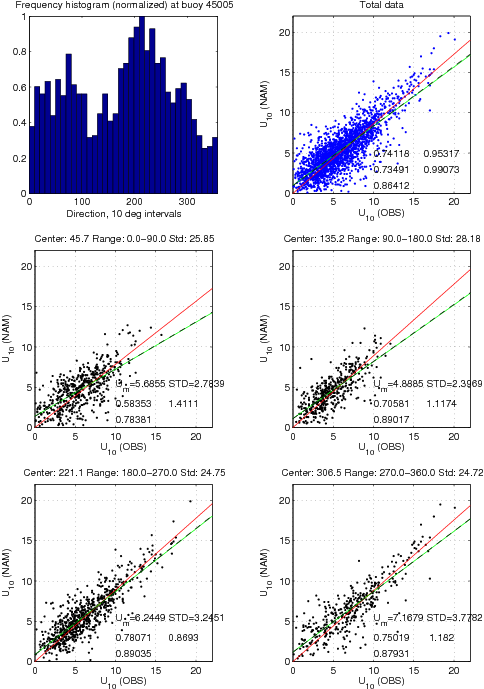
\includegraphics{./figures/fig_45005_4q.png}
 % fig_45005_4q.ps: 490x699 pixel, 72dpi, 17.29x24.66 cm, bb=0 0 490 699
 \label{fig:4q45005}
\end{figure}
 
Bulk assessment of NAM data indicated that surface winds were underestimated at
low wind speeds smaller than 5 m/s, underestimated by 10\% to 20\% in the 5m/s
to 15m/s range and in good agreement for larger intensities. Figure
\ref{fig:nambulk} illustrates the results. Analyses of individual locations
indicated a similar trend, but also revealed the existence of a consistently
higher bias of surface winds near the coastlines. The problem sparkled an
investigation about land-sea boundary issues in the NAM simulations, which will
be explored in more details below. Figure \ref{fig:namshorebias} summarizes the
percentage biases found at selected locations, as a function of distance to the
shoreline.

\begin{figure}[h!]
 \centering
 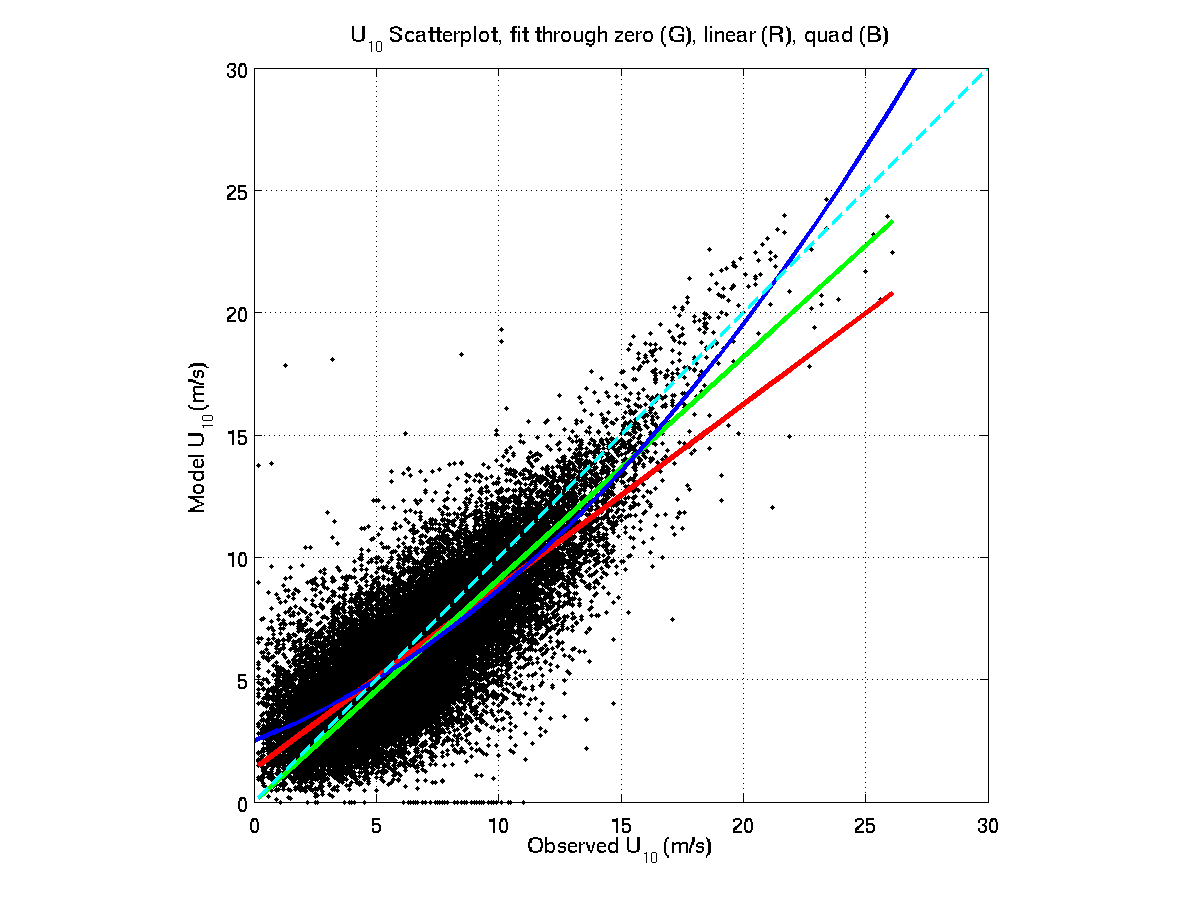
\includegraphics{./figures/fig_nambulk.png}
 % fig_nambulk.eps: 0x0 pixel, 300dpi, 0.00x0.00 cm, bb=
 \label{fig:nambulk}
\end{figure}

\begin{figure}[h!]
 \centering
 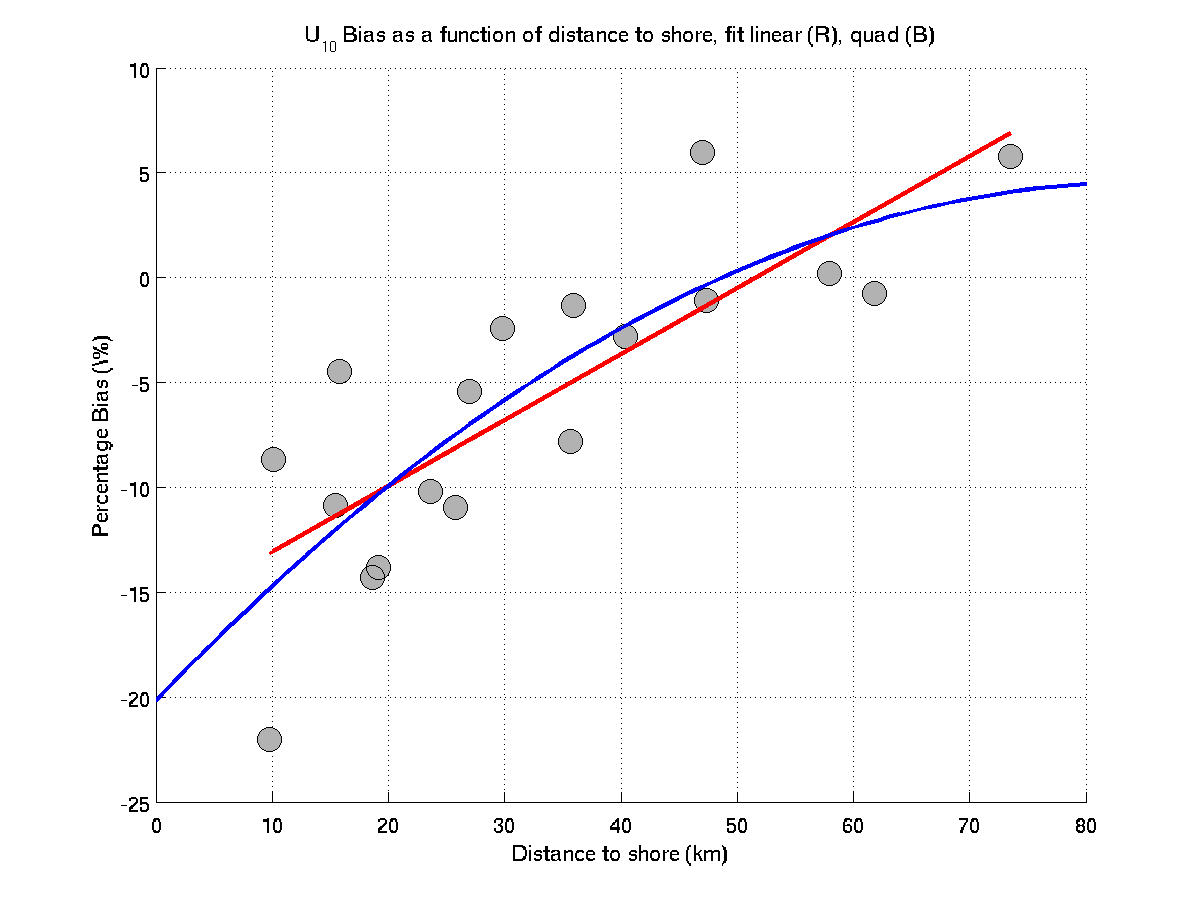
\includegraphics{./figures/fig_namshorebias.png}
 % fig_namshorebias.eps: 0x0 pixel, 300dpi, 0.00x0.00 cm, bb=
 \label{fig:namshorebias}
\end{figure}

Investigations for developing separate strategies for correcting bulk and
distance-to-shoreline biases were initiated independently. Bulk bias correction
was attempted using the average slope of linear regression lines through zero.
Validation statistics indicated that model results were generally insensitive to
the bulk correction, so that a decision was made to go ahead with a future
operational implementation without a bulk surface wind correction component.

A distance-to-shoreline correction scheme was initially envisaged using an
empirical fetch-dependent formula derived from error statistics for NAM surface
winds relative to buoy data. Error maps at selected locations as a function of
wind speed and direction were generated, an illustration of such maps is
provided for station DBLN6 in Figure \ref{fig:nambins}. Global statistics were
then derived from such error maps in an attempt to define a generalized
relationship between wind speed biases and wind fetch geometry. 

\begin{figure}[h!]
 \centering
 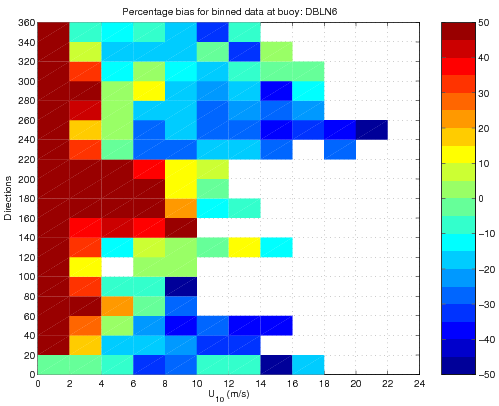
\includegraphics{./figures/fig_DBLN6_bins.png}
 % fig_DBLN6_bins.png: 499x406 pixel, 72dpi, 17.60x14.32 cm, bb=0 0 499 406
 \label{fig:nambins}
\end{figure}

Obtaining generally consistent relationships for correcting wind speeds, based
on fetch geometry, were encouraging. However, the relatively small number of
buoys available in the Great Lakes region, and the fact they are removed during
winter months, limited the reliability of the derived relationships.
Furthermore, as will be explored in more details below, the WAVEWATCH III model
physics, developed mostly for deep-water applications, showed significant
limitations in simulating waves in short-fetch scenarios. 

As a consequence, it was decided that an initial operational implementation of
WAVEWATCH III in the Great Lakes would not include a distance-to-shoreline
correction scheme, until the wave model package included more appropriate
physics to deal with short-fetch wave generation. The correction scheme would be
built based on results summarized above, but would also consider other empirical
and theoretical ideas on land-sea boundary transitions suffered by surface wind
fields. The latter is further discussed below.

\subsubsection{Ice coverage}

The initial operational implementation of the GLW model uses ice concentrations
obtained directly from the NAM atmospheric model data. The latter has a land-sea
mask which is slightly different to that used in the GLW grid, so that
corrections are made. Such correction also account for inconsistencies in ice
coverage close to land boundaries when offshore ice is present at a distance
smaller than a given threshold. If the latter is true, then the ice
concentrations are extended from offshore to the land boundary. The next phases
of upgrades to the GLW system will include high-resolution ice products which
have become available within NOAA/NCEP's operational system.

\subsubsection{Water levels}

Water levels in the Great Lakes show seasonal and longer-term fluctuations. In
both cases, the order of magnitude of water level fluctuations is at 2m. Such
changes may cause differences in wave propagation patterns in nearshore areas.
An assessment of how much water levels affect wave simulations in the region has
been planned, so that future upgrades to the GLW model may include a slow,
seasonal water level variation based on time-averaged gage data for each
individual lake.

